\chapter{xHCI Stack Implementation}

The structure of the xHCI driver is quite straightforward, as it tries to fit
into the scheme of how hardware and the rest of HelenOS works. We decided to
use the existing library \lib{libusbhost} to reduce code duplication with
other HC drivers. It came out that this library need a lot of changes to
support us in this goal, but that's for chapter \ref{usb-refactoring}.

The USB host controller driver using \lib{libusbhost}, xHCI included, serves as
a connecting layer between the hardware and library, and exposes its bus
interface.

\begin{figure}[h]
	\centering
	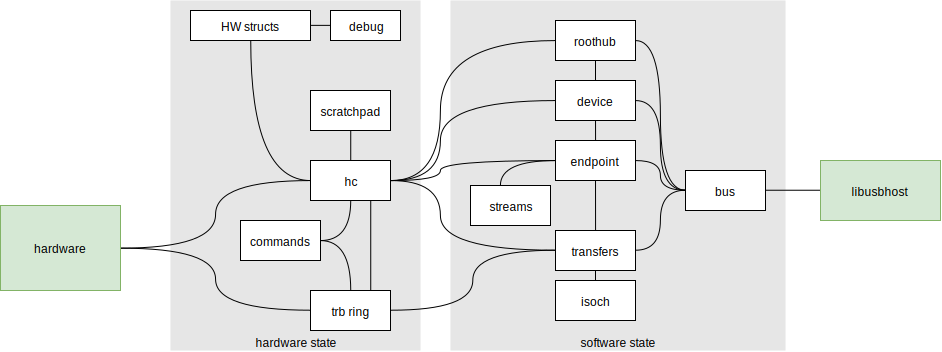
\includegraphics[width=0.8\textwidth]{xhci-architecture}
	\caption{The modules of xHCI driver}
\end{figure}

The scheme is not at all strict, we're in a C world, there are dependencies
almost everywhere -- take it as an informal overview to get an idea.

The whole driver can be split into two parts. The left one takes care about the
hardware perception on what's going on, the right one is about managing the
software structures and memory.

We start with describing the modules in the hardware part, as their
functionality is clear. Their order follows the order in which they were
implemented.

\section{HW structs}

% TODO: Explain that this one is really simple, and just mirrors the structures
% hardware use. Describe briefly the register space of xHC, register field semantics (R, RW, RW1C), contexts.

% TODO @aearsis: Register macros

\section{Debug}

% TODO: Describe that we used it during debugging to check what we're doing.

\section{TRB ring}

% TODO @aearsis: explain the TRB rings, what they do and how they're
% implemented (ْ±2 pages, bore the reader to death right now!)
\subsection{Purpose}
\subsection{Implementation}

\section{Scratchpad}

Scratchpads are buffers that an xHC implementation can request from the system software
for its internal needs. The size of these buffers is specified in the \textit{PAGESIZE} register
found in the operational register set defined in \struct{xhci_op_regs}.

The amount of buffers requested by the xHC is specified in the \textit{Max Scratchpad Bufs Hi} and
\textit{Max Scratchpad Bufs Lo} registers of the second set of structural parameters (\textit{HCSPARAMS2},
see section 5.3.4 of the xHCI specification) defined in \struct{xhci_cap_regs}.

The allocation of these buffers takes place as part of the host constroller initialization,
specifically in \fnc{hc_init_memory()}, which calls \fnc{xhci_scratchpad_alloc()}. The pointers
to these buffers are then passed to the xHC in the \textit{Scratchpad Buffer Array}, pointer to which
occupies the first index of the \textit{Device Context Base Address Array} (dcbaa field of
\struct{xhci_hc_t}).

Our implementation originally implemented these as a standalone structure \struct{xhci_scratchpad_t},
which served mainly for the purposes of resource management by keeping both the physical addresses
for the xHC and the virtual addresses for deallocation. This was, however, later refactored to use
\struct{dma_buffer_t}, which is part of \lib{libusbhost} was created for the same purpose.

Once the xHCI driver finishes its execution, the scratchpad buffers are deallocated by a call to
\fnc{xhci_scratchpad_free()} as part of \fnc{hc_fini()}.


\section{Events}

% TODO: Explain events, event handling and the event ring.

\section{Commands}
\label{sec:commands}

The xHC offers an independent command interface. During operation, the xHC
driver uses this interface to manipulate device slots, devices and endpoints by
executing various commands provided by a unified command subsystem. This
section provides details on the structure and implementation of this subsystem.


\subsection{Execution Workflow}

The xHC command interface consists of a TRB command ring and a command doorbell
register. Commands are executed by placing various command TRBs onto this ring,
forming a \textit{Command Descriptor}.

After placing the respective TRBs and writing to the xHC command doorbell
register, the descriptors on the command ring are sequentially processed by the
xHC, resulting in either failure or successful completion. The result of every
command descriptor is reported back to the xHCI driver in the form of a
\textit{Command Completion Event} placed onto the primary event TRB ring.

After writing into the xHC command doorbell register and before receiving the
respective command completion event, the xHCI driver can attempt to abort the
issued command. Such action might be of use for instance if the command
completion event does not arrive within a set time period.

Note that this section intentionally omits hardware technical details, which are
not instrumental in understanding the command subsystem. For further hardware
documentation of the xHC command interface, refer to \xhci{4.6}.


\subsection{Structure}

The xHCI driver command subsystem instance is represented by the
\struct{xhci_cmd_ring_t} structure which exists throughout the entire duration
of the xHCI driver's lifecycle. The purpose of this structure is to maintain and
manage the command TRB ring and to keep track of enqueued command descriptors.

Individual command descriptors are represented by the \struct{xhci_cmd_t}
structure. In this structure are stored high-level parameters of the command as well as
the command TRB, which is placed onto the command ring when the command is
executed. While the high-level command parameters are kept directly in this
structure, the hardware-related internals are kept in a substructure, which is
commonly referred to as \textit{command header}. The purpose of this separation
is to stress that the header contents are to be exclusively accessible to the
command subsystem, while the rest of the structure remains accessible to
the entire xHCI driver.

Besides data structures, the command subsystem offers a centralized command
completion event handler function -- \fnc{xhci_handle_command_completion} --
which is called by the event subsystem in case a \textit{Command Completion
Event} is encountered.

The last major component of the command subsystem are functions used to generate
and schedule commands on the xHC. These functions produce valid instances of the
\struct{xhci_cmd_t} and place their respective TRBs onto the command ring
managed by the \struct{xhci_cmd_ring_t} structure, requesting either blocking or
non-blocking semantics for waiting on their completion. These functions are
described in detail in the next section.


\subsection{Command Lifecycle}

\subsubsection{Issuing Commands}

By design, the internal logic of the command subsystem is kept opaque with
respect to other components of the driver. A notable example of this is the
mechanism for command scheduling.

Commands are usually issued by the HC component of the xHCI driver. At the time
of issuing, the information required can be broken down into three groups:
%
\begin{description}
	\item[Command Type]
		One of the 15 commands supported by the xHC command interface.
	\item[Command-specific Parameters]
		The number, type and semantics of these parameters depend on the
		specified command type.
	\item[Completion Semantics]
		This is the desired behavior of command execution.

		In the \textit{blocking mode}, the call to issue the command will block
		the calling fibril until the completion event is received.

		On the other hand, in the \textit{non-blocking mode}, the fibril will
		only be blocked until the command is issued -- the command subsystem
		will take the ownership of the command and deallocate it when the
		completion event arrives. This mode is meant for commands which do not
		require completion event handling and involves more complicated memory
		management since the command subsystem is responsible for freeing the
		command after the completion occurs.
\end{description}

Depending on the desired completion semantics of the issued command, the HC
component calls either the \fnc{xhci_cmd_sync} or \fnc{xhci_cmd_async}
function and passes it a configured instance of the \struct{xhci_cmd_t} structure.
Upon such call, the command subsystem will execute an internal command handler
function, which copies the high-level command-specific parameters configured by
the issuer, and use their values to construct a command descriptor consisting of
TRBs.

At this point, the \struct{xhci_cmd_ring_t} structure is modified and the new
command descriptor is placed onto the TRB ring. The corresponding instance of
\struct{xhci_cmd_t} is added to the active command list and depending on the
completion semantics, the issuing fibril is either suspended or continues
execution regardless of the completion event.


\subsubsection{Handling Completion}

When a command is completed, a \textit{Command Completion Event} is generated by
the xHC. This event is detected by the event subsystem, which in such case
triggers the \fnc{xhci_handle_command_completion} function.

This function extracts the address of the completed command descriptor and uses
it to find a matching instance of the \struct{xhci_cmd_t} structure in the
active command list.

Depending on the desired completion semantics, the command subsystem either
wakes the sleeping issuer fibril, or discards the non-blocking command from the
memory.


\subsubsection{Aborting Commands}

The command subsystem defined by xHCI contains a mechanism to trigger early
command abortion. It is not guaranteed to be effective for all commands, just
for commands control of which is out of HC's hands. A good example might be the
\macro{SET_ADDRESS} command, which issues the USB control request
\emph{SetAddress}, and waits for the device's response. Such command blocks
until the response is received. If the software, for any reason, wants the
command to be aborted, it can write 1 to the \macro{CA} bit of the
\emph{Command Ring Control Register}.

When the HC is triggered by a command abortion, it places a \emph{Command Ring
Stopped} event on the primary event ring and halts command processing. The ring
can be started again by ringing its doorbell. If a command was actually
aborted, a corresponding \emph{Command Completion Event} with status
\emph{Command Aborted} is placed first.

We decided to set a fixed timeout for every command, regardless of its
possibility to block, arbitrarily chosen as 10 seconds. That gives a generous
amount of time for the HC to finish a command. When this timeout is over,
a command is aborted.

Here comes the catch: the driver is not able to choose which command is to be
aborted -- it is always the one currently processed. Usually, it's the one that
blocks the pipe, but it means that the driver cannot simply place a timed
constraint on a command execution. To reflect the hardware semantics, all
fibrils that expire the timeout behave the same: they trigger a command
abortion, wait for the command ring to be stopped, then start it again.

To orchestrate several fibrils trying to schedule new commands, waiting for
commands to be completed and also the one handling an interrupt, a simple state
machine with synchronization is incorporated. In case the command ring is
being restarted, newly issued commands are delayed to prevent the doorbell from
being rung unexpectedly. When there are multiple fibrils with an expired timeout
while the abort is already triggered but not yet finished, they retract and
wait for the full timeout period again.

That common execution path is enclosed within a function called
\fnc{try_abort_current_command} (static for the command subsystem). As it's hard
to force a command to stall, we haven't had many opportunities to test the
behavior. Usually, the mechanism was triggered by a deadlock in our code, which
didn't magically disappear when a command was aborted. Also, the commands
always finish on time in a virtual environment. At the time of writing this
documentation, there has been only one observed legitimate occurrence of
a command stall on real hardware. The abort mechanism did its job well that day.

\subsection{Usage Examples}

Since the command subsystem is used at a multitude of places in the HC
component, it has been the goal of the authors to make its usage elegant and
effortless. For that reason, a dedicated inline notation syntax powered by
preprocessor macros has been devised and implemented. This is demonstrated in
Listing \ref{lst:command-usage}.

\begin{listing}[h]
	\begin{code}
		xhci_hc_t * const hc;

		/* Issue a "Set TR Dequeue Pointer" command synchronously. */
		const int result = xhci_cmd_sync_inline(hc, SET_TR_DEQUEUE_POINTER,
		    /* Command-specific arguments use struct initializer. */
		    .slot_id = slot_id,
		    .endpoint_id = dci,
		    .stream_id = stream_id,
		    .dequeue_ptr = addr,
		);

		/* At this point, the command is completed with `result`. */
	\end{code}
	\caption[Usage example of xHCI driver inline command syntax.]{Usage example
	of the xHCI driver command subsystem inline  syntax. This snippet issues a
	\textit{Set TR Dequeue Pointer} command to the HC in blocking mode. Note
	that the command initialization, configuration and finalization is handled
	by the inline macro syntax.}
	\label{lst:command-usage}
\end{listing}



\section{Host controller module}

% TODO: This will be harder, this one is a mix of what didn't fit anywhere else.
% Ideas:
% - event handling
% - context management
% - extcap parsing
\
\section{Roothub}

The purpose of this module is very simple -- take care of the root hub. Before
we explain how our roothub works, let's have a look on why and how other HC
drivers' handle it.

The main problem a hub driver faces is a synchronization one. When a new device
is detected, it needs to be enumerated. Enumeration process in case of USB 2.0
devices requires the hub to reset the port the device is attached to, to move
it the \textit{Default} state, when it's listening on the default address 0.
Wen the port reset is triggered, the hub must wait until the port reset is
complete. During the whole process, the device can be disconnected, and the
port reset will never be completed. Furthermore, the completion of port reset
is indicated by the same means as port connection, resulting in a deadlock in
the na\"ive solution. The proper solution therefore involves spawning new
fibrils and nontrivial synchronization.

All four HC drivers (UHCI, OHCI, EHCI and VHC) are using a virtual roothub. In
principle that means that they create a virtual USB device, which is listening
at the default address in the beginning, and trigger an enumeration process.
Then there is a little branch in transfer scheduling, that takes transfers
directed to the same address as the virtual device's, and delivers them by
calling a function instead. The virtual device behaves exactly like a real USB
hub would -- it has its standard descriptors, reply to setup requests and so
on. So it enumerates like a USB hub would, and creates a DDF device, which is
taken by the \texttt{usbhub} driver. The driver then handles the virtual
roothub like any other hub, by sending USB control transfers. The virthub
module translates USB transfers to callbacks, which are implemented by
individual HC driver to read and modify register space of the Host Controller.

This solution is very clean in design, regarding that root hub functionality is
exactly the same as any other hub's, it is just controlled by MMIO mapped
registers instead of USB packets. It is even recommended by the USB 2.0			% TODO: Link to USB2 spec
specification to embody this solution. But that's pretty much the only advance
this solution has. One has to write a lot of code to even implement the
callbacks, not mentioning the virthub module itself. And a lot of code always
come with bugs. Also, while having no real performance impact, it requires
several context switches, IPC calls, bouncing memory buffers and a lot of
unnecessary allocations to clear one bit in the register space (USB hubs
operate by setting and clearing so called Features, indicating e.g. that
a connection on port changed). But it needs to be stressed more, that this
performance impact is mitigated by the fact real hub use real USB transactions
above that, and that hub interaction is very sparse.

We searched for solution, that would keep the cleanness in terms of shared
functionality between usbhub driver and roothub, and decided to move the port
state machine and related fibril synchronization into the USB library. That
cleanly separates the hardest part of handling hub port changes from the code
that is actually handling them and enumerating the devices. This state machine
is used by both xHCI roothub, and also by the rewritten usbhub. More
information about this new module can be found in section \ref{hub-port-refactoring}.

One more thing related to the xHCI roothub, which we crossed while debugging on
real hardware. The USB hub have a bit dedicated to indicate that a port is
enabled (PED), and the port can be disabled using it. Counterintuitively, the
port is disabled by writing a 1 to it. Even worse, this bit is in the same
field as the change bits with RW1C semantics are -- which means that the
standard approach of reading and writing back the value read fails hard. This
took us several hours to discover, because the port reset was completed
successfully, but right after that, the device was inaccessible, even when we
didn't do anything with it yet. To make matters more complicated, QEMU ignores
this bit completely, so the code worked fine in a virtual environment.


\section{Transfers}

% TODO @salmelu (probably?): Write something about it.

\subsection{Isochronous transfers}

% TODO @salmelu: Copy that from the wiki :)

\section{Bus module}

% TODO: After the device will be split, will there be anything interesting to write about?

\subsection{Device}

% TODO: Enumeration, device context

\subsection{Endpoint}

% TODO: Contexts, rings

\subsection{Streams}

% TODO @salmelu: Noone else understands that now.
